% GigaScience template
\documentclass[a4paper,num-refs]{oup-contemporary}

\journal{gigascience}


%%%% Packages %%%%
\usepackage{siunitx}
\usepackage{minted} % Used for JSON highlighting
\usepackage{algpseudocode} % Algorithmic environment
\usepackage{xspace}
\usepackage{booktabs}

%%%%%%

\usepackage{xcolor}
\usepackage{graphicx}
\usepackage{algorithm}
\usepackage{caption}
\usepackage{subcaption}
\usepackage{listings}
\usepackage{verbatim}
\usepackage{makecell}
\usepackage[flushleft]{threeparttable}

\usepackage{subcaption}
\usepackage{xspace}
\usepackage{stmaryrd} % for llbracket and rrbracket
\usepackage{amsmath}
\usepackage{ulem}
\DeclareMathOperator*{\argmin}{argmin}

%%%% Commands %%%%
\newcommand{\todo}[1]{\color{red}\textbf{TODO:}#1\color{black}}
\newcommand{\note}[2]{\color{blue}Note: #1\color{black}}
\newcommand{\reprozip}[0]{ReproZip\xspace}
\newcommand{\tristan}[1]{\color{blue}\textbf{From Tristan:}#1\color{black}}
\newcommand{\english}[1]{\uwave{#1}}

 
\title{NURM: a tool to 
locate numerical differences in pipelines}
  
\begin{document}

\author[1]{Ali Salari}
\author[1]{Lalet Scaria}
\author[2,3]{Gregory Kiar}
\author[2]{Lindsay Lewis}
\author[2,3]{Alan C. Evans}
\author[1]{Tristan Glatard}

\affil[1]{Department of Computer Science and Software Engineering, Concordia University, Montreal, Canada}
\affil[2]{McGill University, Montreal, Canada}
\affil[3]{Montreal Neurological Institute, Montreal, Canada}

\maketitle

\begin{abstract} 

Many experiments show that computational analysis results are still not 
completely reproducible. Computational environments including different 
operating systems, hardware categories, and software versions are known 
to have effects on the results produced by analysis pipelines. These 
effects are presumably due to the creation, propagation and 
amplification of small numerical differences across the pipelines. 
Although new techniques such as virtualization, version control 
systems, and provenance management tools provide a more reliable 
environment and significantly improve the reproducibility of scientific 
findings. However, the precise causes of such instabilities and the 
path along which they propagate in the pipelines are unclear.  We 
present a technique to identify the processes in the pipeline that 
create numerical differences along with the execution, and we apply this 
technique to the HCP structural pre-processing pipelines.

\end{abstract}

\begin{keywords}
Reproducibility; Numerical Instability; Neuroimaging.
\end{keywords}

\section{Introduction}

Reproducibility is a crucial element of the scientific works, 
as it enables researchers to evaluate authenticity and reliability 
of the findings~\cite{plesser2018reproducibility}.
Reproducibility is defined as the ability to regenerate the same 
results as the original findings when the experiment is reanalyzed by 
the same analytic methods, software package, parameters, and 
data~\cite{peng2011reproducible}. 
In addition, numerical reproducibility is defined as the ability to 
regenerate bit for bit identical results from multiple 
runs~\cite{hill2017numerical}. 
We considered the numerical reproducibility in our experiments by comparing 
the binary content of the results using the checksum method.

Recently, validation of the reproducibility has been widely investigated 
in the field of neuroimaging in which uses optimized 
processing methods with the purpose of functional and structural 
assessments of the human brain.
According to the previous 
studies, the variety of computing infrastructures including workstation 
types, parallelization methods, operating systems, and analysis 
packages are known to influence the reproducibility of the analyses~\cite{Gronenschild2012, 
diethelm2012limits, Glatard2015, bowring2019exploring}.

In particular, the studies on the effect of the operating system on the results show that 
computational pipelines create small numerical differences~\cite{Glatard2015, Scaria2017}.
These differences mainly correspond to the mathematical functions implemented 
in different operating system libraries.
For instance, changing the mathematical functions like \emph{expf()} and 
\emph{cosf()} which manipulate the precision of floating-point representations, 
between \emph{glibc} libraries in different operating systems can produce 
small numerical differences.
Besides, a similar issue is expected for any operating system which is 
based on \emph{glibc}, the GNU C library.

These irreproducibility issues are reported as the result of the 
creation, propagation, and amplification of small numerical 
differences~\cite{Gronenschild2012, diethelm2012limits, Glatard2015, 
bowring2019exploring}. In this case, the analysis pipelines are said to 
be numerically unstable. Numerical instability is a characteristic of 
the pipelines which amplify small numerical differences and then hamper 
the reproducibility of the analyses depending on the length of the 
pipeline and magnitude of the differences. In many cases, numerical 
instability is an essential issue for reproducibility.

There are different solutions to improve the reproducibility of the analysis, 
including containerization techniques that encapsulate software/hardware 
dependencies, provenance capturing tools, and version control systems. 
However, a comprehensive solution requires to fix the numerical 
instabilities instead of masking the issue. For this purpose, we introduce 
the Numerical Reproducibility Measurement (NURM) tool to identify the processes in 
the pipeline that create numerical differences across several runs. 
Furthermore, we can fix the instability of the identified processes 
in the next steps.

The remainder of this paper describes the NURM-tool in different parts 
including the way of capturing and representation of the provenance 
information, the method of clustering of different subject types, and 
process labelling to characterize differences. We describe the HCP 
preprocessing pipelines as a popular neuroimaging project to test the 
NURM-tool and evaluate its functionality. Finally, we reported the 
experimental results which describe the processes that are responsible 
for the differences in the pipelines.

\section{Tool description}

Figure~\ref{fig:overview} shows an overview of our method. For each tested
condition, Condition 1 and Condition 2, the pipeline is containerized with
Docker, and its interface is described with
Boutiques~\cite{glatard2017boutiques}. \reprozip~\cite{chirigati2016reprozip} is
added to Condition 1 for provenance tracking. Our tool starts by
identifying temporary files and ``multi-write" files, i.e., files written
by more than one process (Figure~\ref{fig:overview-capturing}). To do that,
the tool first executes the pipeline in Condition 1, to obtain a process
graph (Figure~\ref{fig:overview-capturing} - (1)) and a list of result files.
The list of processes that create intermediary or multi-write
files is then generated (Figure~\ref{fig:overview-capturing} - (2)). 
Using this list, the tool modifies Docker image in Condition 1 and
exectutes the pipeline again through it, which turns to produce results
including temporary and overwritten files
(Figure~\ref{fig:overview-capturing} - (3,4)). In the second step, the
processes are labeled from the differences found in their outputs in the
two tested conditions (Figure~\ref{fig:overview-labelling}). To this order,
the tool builds docker image for Condition 2 by modifying pipeline
processes (Figure~\ref{fig:overview-labelling} - (1)) that recognised from 
the process graph. Then, the modified docker
image is executed in Condition 2 and each process is labeled right after
the running by comparing the results obtained in Condition 1
and output files of the process in Condition 2
(Figure~\ref{fig:overview-labelling} - (2)). We then label processes in 2
categories depending whether they
create differences (represented in red) or not (green). 
The tool replaces output file with the same file obtained in Condition 1 
if process creates differences (Figure~\ref{fig:overview-labelling} - (3)).
Process labelling
is done through hooks which are defined during the docker image modifying
procedure, and incremental updates in Condition 2, until the end of the
pipeline execution.

\begin{figure}
  \centering
  \begin{subfigure}{\columnwidth}
    \centering
    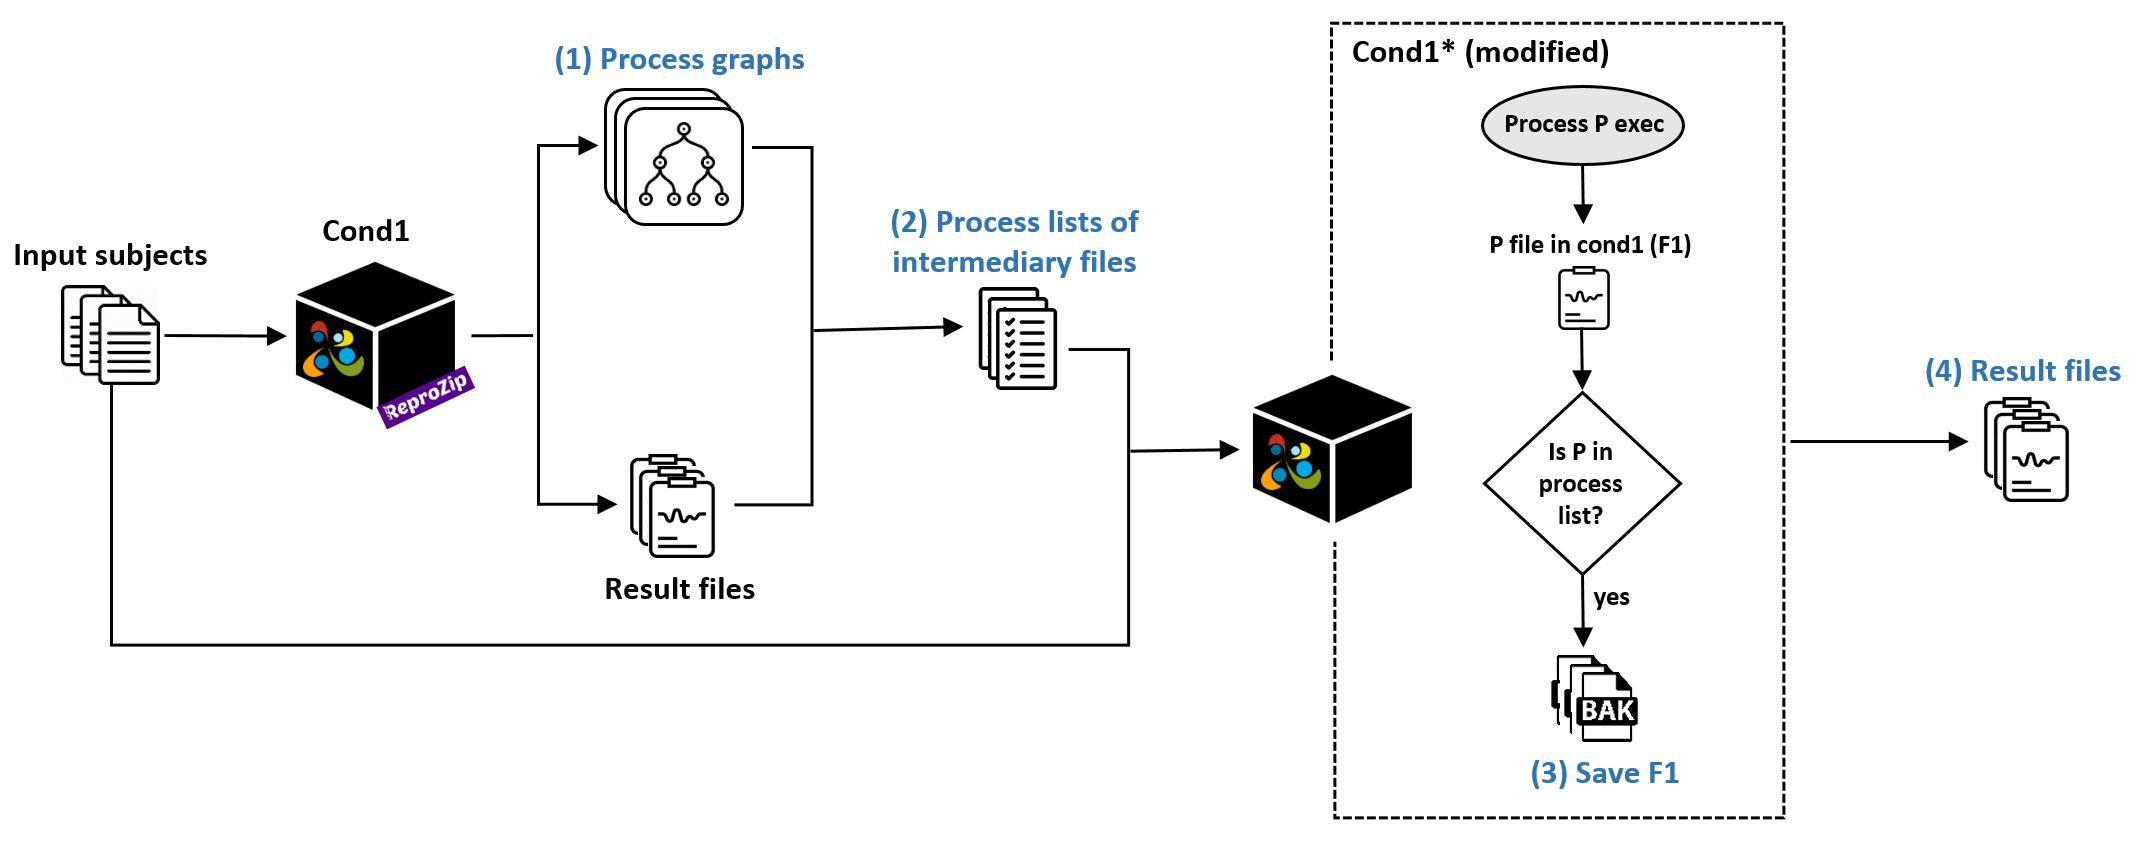
\includegraphics[width=1\columnwidth]{images/fig1-a}
    \caption{Identification of temporary and multi-write files.
    (\href{https://docs.google.com/drawings/d/1rsbFwPjNPNMRhXUl4RSK3G0OaiJC7K-buiHN0hPD8eQ/edit?usp=sharing}{Source})}
    \label{fig:overview-capturing}
  \end{subfigure}
   \begin{subfigure}{\columnwidth}
    \centering
     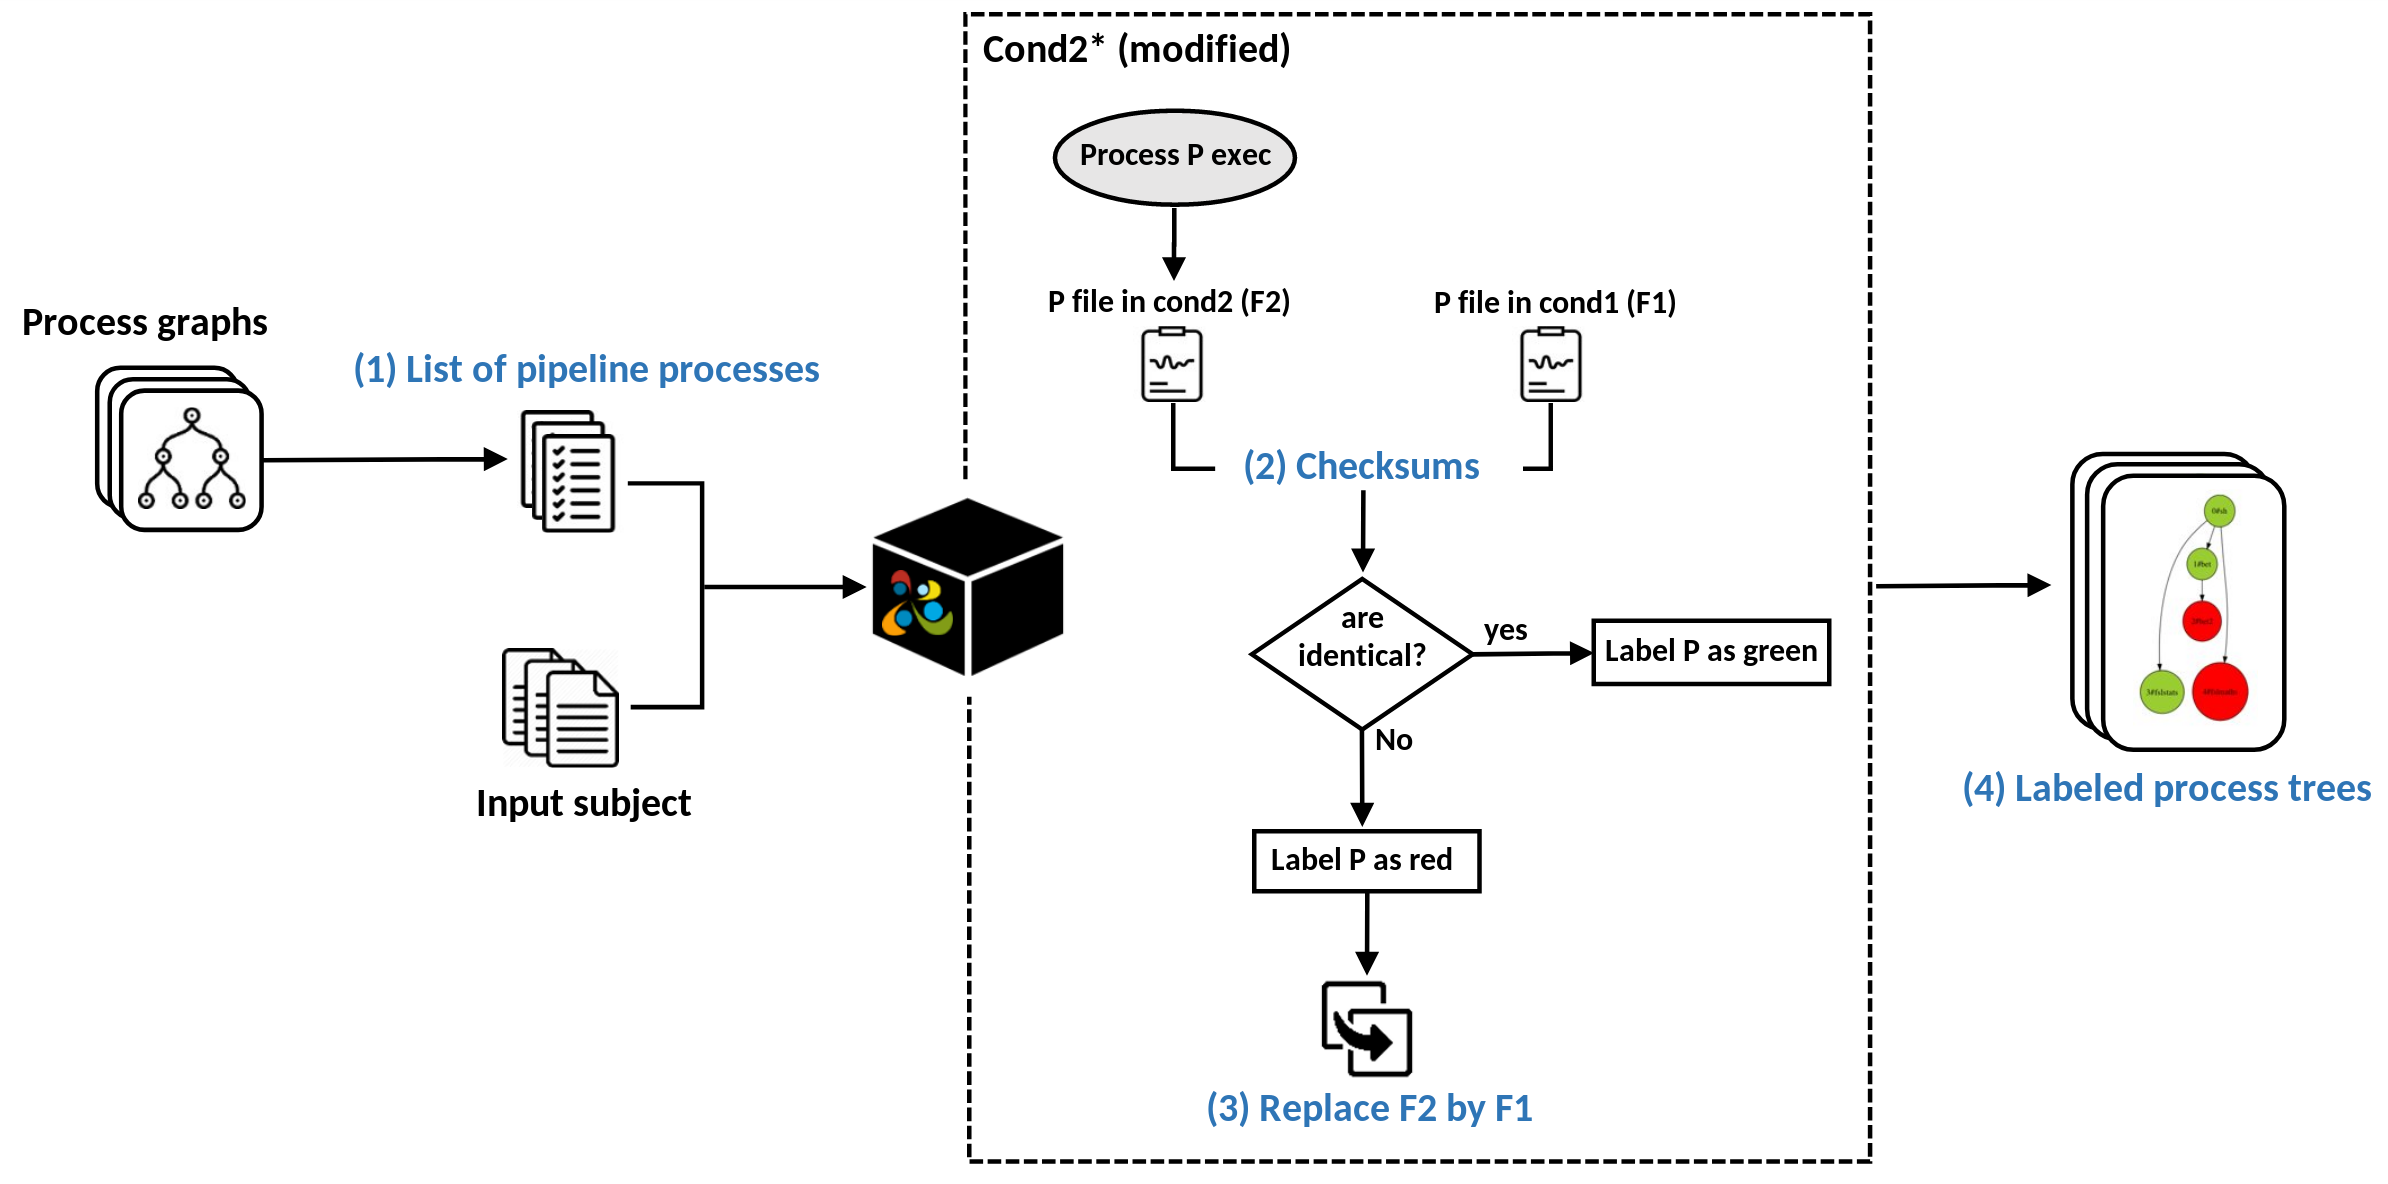
\includegraphics[width=1\columnwidth]{images/fig1-b}
     \caption{Labelling process graphs including intermediary files.
     (\href{https://docs.google.com/drawings/d/1yblYuKWAD18aJe5JxBu2h1EysyoQA3YrsQj-1T3s0l8/edit?usp=sharing}{Source})}
     \label{fig:overview-labelling}
   \end{subfigure}
   \caption{An overview of NURM-tool in two steps. First capturing intermediary files (a); then
            labelling process graphs (b).}
   \label{fig:overview}
  \end{figure}

\subsection{Provenance capture and representation}

We use \reprozip 
to capture: (1) the set of processes created by the
pipeline, using the \texttt{clone()} or \texttt{fork()} system call, and
(2) the set of files read, written and executed by each process, including
temporary files. \reprozip collects this information through the
\texttt{ptrace()} system call and stores it in a SQLite database.

Our tool reconstructs a \emph{process tree} starting from the first process
created by the pipeline and traversing processes through \texttt{clone()}
and \texttt{fork()} dependencies. Our tool also creates a process \emph{graph} 
(Figure~\ref{fig:overview-capturing} - (1)) from this tree
by adding edges corresponding to file dependencies between processes. A
file dependency is defined between processes A and B if a file written by A
is read by B. Figure~\ref{fig:simple_script} shows an example of a process
tree and graph constructed from the example pipeline in
Listing~\ref{listing:sample-script}.
\begin{listing}
\begin{minted}[frame=single,
  framesep=3mm,
  linenos=false,
  xleftmargin=0pt,
  tabsize=4]{bash}
#!/bin/bash

# This script extracts the brain from an input image,
# measures the volume of the extracted brain,
# and creates a binarized brain mask.

if [ $# != 1 ]
then
    echo "usage: $0 <inputimage.nii.gz>"
    exit 1
fi

# Parse argument, set file names
input_image=$1
bet_output=$(basename "${input_image}" \
                       .nii.gz)_brain.nii.gz
bet_output_binarized=$(basename "${input_image}" \
                       .nii.gz)_brain_bin.nii.gz

# Run FSL bet, put result ${bet_output}
bet "${input_image}" "${bet_output}" > bet_temp.out
echo "Voxels / Volume in brain mask:"
# Run FSL stats on ${bet_output}
fslstats "${bet_output}" -V
# Run FSL maths on ${bet_output}
fslmaths "${bet_output}" "${bet_output_binarized}"
# Remove temporary file
\rm bet_temp.out
\end{minted}
  \caption{Example pipeline}
  \label{listing:sample-script}
\end{listing}

\begin{figure}
\centering
  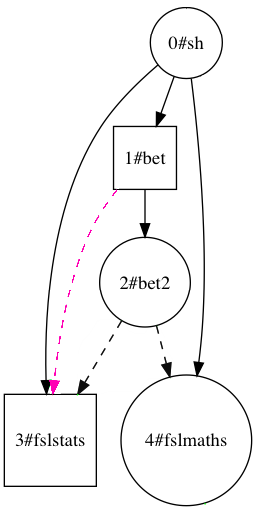
\includegraphics[width=0.3\columnwidth]{images/simple_graph}
  \caption{Process tree and graph
  constructed from the example pipeline in
  Listing~\ref{listing:sample-script}.
  Processes that read or write
  temporary files are 
  represented with squares. Plain edges 
  represent the process tree (\texttt{fork()} or \texttt{clone()} 
  system calls). Dashed edges represent file dependencies: temporary 
  files are in yellow and result files are in green.
  Every node in the tree is labeled using (1) a process id created by our
  reconstruction, (2) the name of the executable run by the process.
  Process 0 is the initial call to the \texttt{sh} interpreter, and
  processes 1, 3 and 4 are the calls to FSL bet, stats and maths made in
  Listing~\ref{listing:sample-script}. Process 2 is forked by process 1: it
  was captured by \reprozip while it did not appear in
  Listing~\ref{listing:sample-script}. 
}
  \label{fig:simple_script}
\end{figure}


\subsection{Graph analysis}

We label in two categories the processes of the graph of each subject. First,
processes that read files that do not have differences and write files that
do not have differences are labeled \emph{transparent}
(Figure~\ref{fig:green}). Second, processes that read files that do not
have differences but write files that have differences \emph{create}
differences (Figure~\ref{fig:red}). In addition, processes that read files
that have differences and write files that also have differences are called
\emph{undetermined} (Figure~\ref{fig:yellow}). Processes are also labeled
undetermined when they read or write temporary files, or produce multi-write
files. To resolve undetermined processes, hooks must be added to the pipeline to 
execute these processes on files without differences, and to capture
intermediary file states.

\begin{figure}%\centering
\centering
    \begin{subfigure}{0.2\linewidth}
        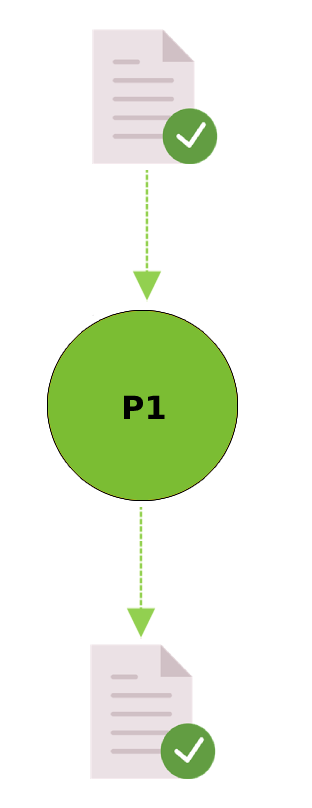
\includegraphics[scale=0.3]{images/green.png}
        \caption{Transparent}
        \label{fig:green}
    \end{subfigure}
    \hfill
    \begin{subfigure}{0.2\linewidth}
    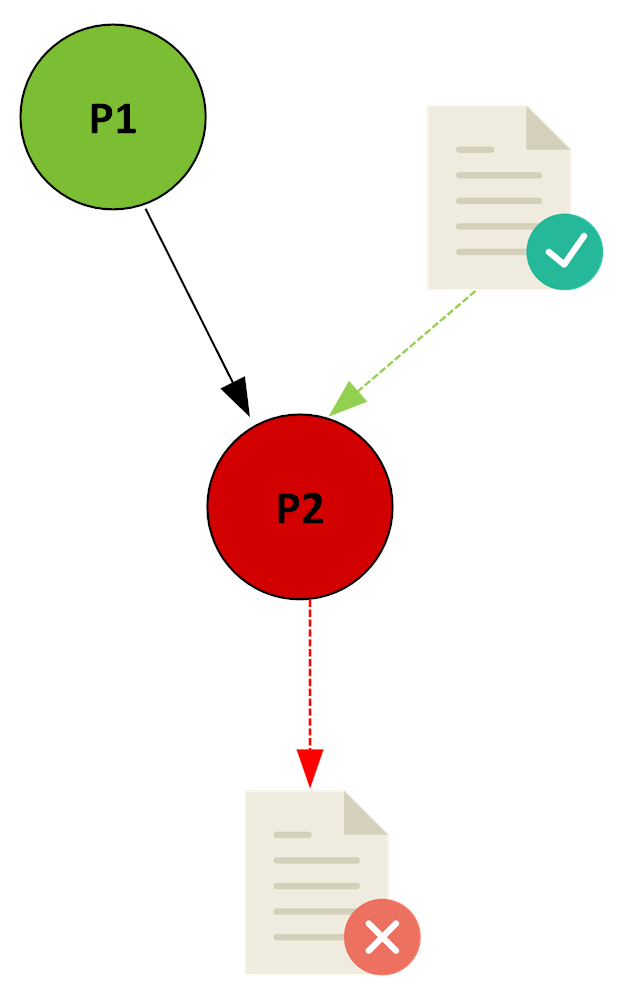
\includegraphics[scale=0.3]{images/red.png}
    \caption{Creates differences}
    \label{fig:red}
    \end{subfigure}
    \hfill
    \begin{subfigure}{0.2\linewidth}
    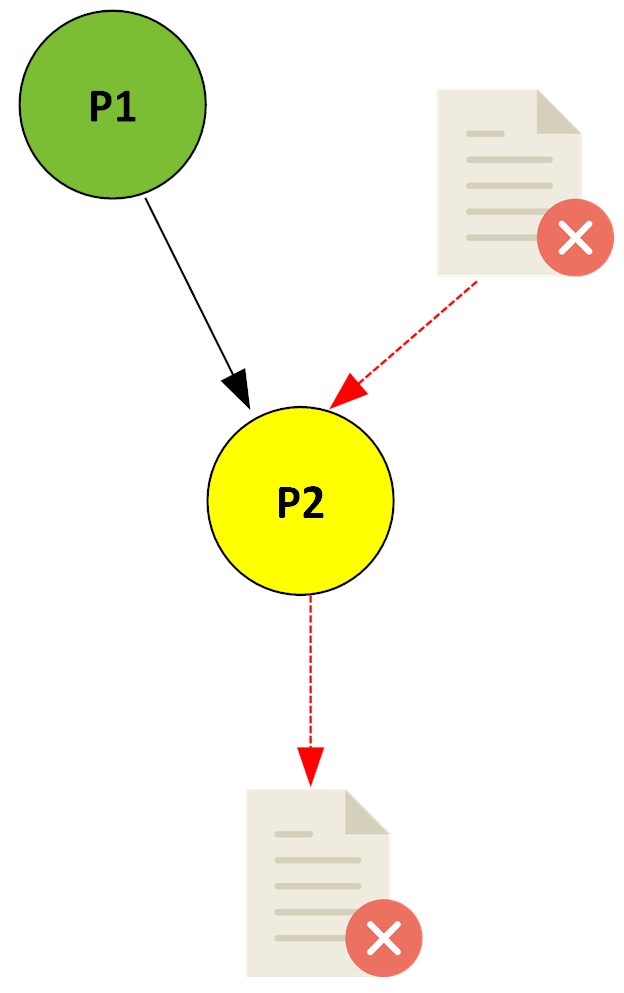
\includegraphics[scale=0.3]{images/yellow.png}
    \caption{Undetermined}
    \label{fig:yellow}
\end{subfigure}
    \caption{Different type of labeled process based on the input/output files.
  Dashed edges refer to the file dependencies between processes A and B 
  if a file written by A is read by B. Solid black edges refer to the 
  relationship between parent and child processes.}
    \label{fig:processes}
\end{figure}

\subsubsection{Capturing temporary files} 

The label of processes that read or 
write temporary files is undetermined because these files are deleted during 
the execution. To address this issue, we replace in Condition 1 every process P that 
writes temporary files by a wrapper that first calls P and then
saves all its output files to a read-only directory. This replacement is
done by modifying the PATH environment variable to point to a directory
containing a modified version of the executable called by the process. The
modified executable will run the original executable and then save its
output files (see Listing~\ref{listing:modify-script}). 
This 
solution does not cover the temporary files that are removed by P 
itself, but this is not a problem since these files do not play any role in 
the subsequent steps of the pipeline. 

\begin{listing}
  \begin{minted}[frame=single,
    framesep=3mm,
    linenos=false,
    xleftmargin=0pt,
    tabsize=4]{python}
  #!/usr/bin/env python
  import os.path as op
  import shutil
  import pipes

  # Run the original executable using the same arguments
  executed_file = sys.argv[0]
  exec_argv = op.join('original_scripts', executed_file)
  exec_argv = exec_argv + " ".join(map(pipes.quote, sys.argv[1:]))
  subprocess.Popen(exec_argv, shell=True).communicate()
  
  # Load list of captured process to be checked
  with open('path/to/p_list/', 'r') as p_list:
      process_list = json.load(p_list)

  if exec_argv in process_list.keys():
      # Save output files to read-only directory
      p_files = process_list[exec_argv]
      shutil.copy(p_files, '/read-only/dir')
  
  \end{minted}
    \caption{Modified version of the script in Listing~\ref{listing:sample-script} to save intermediary files.}
    \label{listing:modify-script}
  \end{listing}

\subsubsection{Capturing multi-write files}

Files written by multiple processes also lead 
to undetermined labels. For a file F 
written by all processes in \textbf{P} = \{$P_{1}$, \ldots $P_{n}$\}, we 
(1) check that processes in \textbf{P} do not write concurrently to F, 
(2) we establish an order on \textbf{P} based on the creation timestamp 
of the processes, (3) we replace every process $P_{i}$ in \textbf{P} by 
a wrapper that first calls $P_{i}$ and then saves F to a read-only 
directory. Thus, multiple versions of F are saved and used in the 
analysis. 

Furthermore, cycles may be present in the process graph in case a file 
was written by more than one process. We remove such cycles by removing 
file edges between processes A and B when A's process creation 
timestamp is posterior to B's or when A=B. Indeed, such edges cannot 
happen in practice unless A and B were running concurrently, which we 
assume is not the case (the tool checks for that). 

As an example of this capturing process, in the sample pipeline in 
Listing~\ref{listing:sample-script}, process \texttt{2\#bet2} writes a temporary file and 
also file \emph{T1w\_brain\_bin.nii.gz} is first written by process \texttt{2\#bet2} and 
then overwritten by process \texttt{3\#fslmaths}. The list of these processes is captured in 
Listing~\ref{listing:json_process}.
Using this list, we modify relevant processes in Condition 1 and then re-execute pipeline 
to save them in a backup folder.
Figure~\ref{fig:overview-capturing} - (4) shows pipeline results including intermediary files 
captured as the outputs in Condition 1. 

\begin{listing}
  \begin{minted}[frame=single,
    framesep=3mm,
    linenos=false,
    xleftmargin=0pt,
    tabsize=4]{JSON}
{
  "multi_write_process": {
    "fslmaths\00T1w_brain.nii.gz\00T1w_brain_bin.nii.gz":
    {
      "files":[
        "/cond1/subj1/T1w_brain_bin.nii.gz"
      ],
      "pid": 78
    },
    "bet2\00/cond1/subj1/T1w.nii.gz\00T1w_brain.nii.gz":
    {
      "files":[
        "/cond1/subj1/T1w_brain_bin.nii.gz"
      ],
      "pid": 75
    }
  },
  "temp_process": {
    "bet2\00/cond1/subj1/T1w.nii.gz\00T1w_brain.nii.gz": 
    {
      "files": [
        "/cond1/subj1/temp.tmp"
      ],
      "pid": 75
    } 
  } 
}

\end{minted}
\caption{List of process and their files from the example pipeline in 
Listing~\ref{listing:sample-script} that should be captured.}
\label{listing:json_process}
\end{listing}


\subsubsection{Labelling undetermined processes} 

Since all the result files are captured in Condition 1, the tool 
is ready to label the piepeline processes based on the results in Condition 2.
However, another challenge is to label undetermined processes that read files with 
differences and write files with differences too. In this
situation, it is not possible to determine from the pipeline results 
whether the process created differences or 
was transparent.
To address this issue, we set hooks in the pipeline 
in Condition 2. Hooks are set by replacing the pipeline 
processes with a custom script. This custom script labels each process 
as \emph{transparent} or \emph{create differences} immediately after running 
the original executable. 
The replacement is done through the PATH variable, as before. Moreover, 
this custom script copies the results obtained from the same process in 
Condition 1 to the pipeline output in Condition 2 if 
it is invoked with the arguments of a process that created differences 
(Figure~\ref{fig:overview-labelling} - (3)). 
Differences are identified by comparing checksum of the output files for 
the same process in both conditions (Figure~\ref{fig:overview-labelling} - (2)).
In addition, the distance functions that are specific to file types can be added 
to our tool to ensure that differences belong to the file data part.
We developed an incremental approach that consists of the following steps: 

\begin{enumerate}
  \item Start the pipeline execution in Condition 2; 
        after hooking all the processes involved in the pipeline.
  \item Label each process as \emph{transparent} or \emph{create differences} 
        right after its running.
  \item Check if process is \emph{create differences} then: 
        copy the results produced by the same process in Condition 1 to the 
        pipeline output in Condition 2. 
  \item Continue steps 2 and 3 until the end of the pipeline execution.
\end{enumerate}

This algorithm creates a \emph{labeled process tree} at the end of pipeline execution 
which highlights processes that create differences.
(Figure~\ref{fig:overview-labelling} - (4)).

\begin{figure}
  \centering
  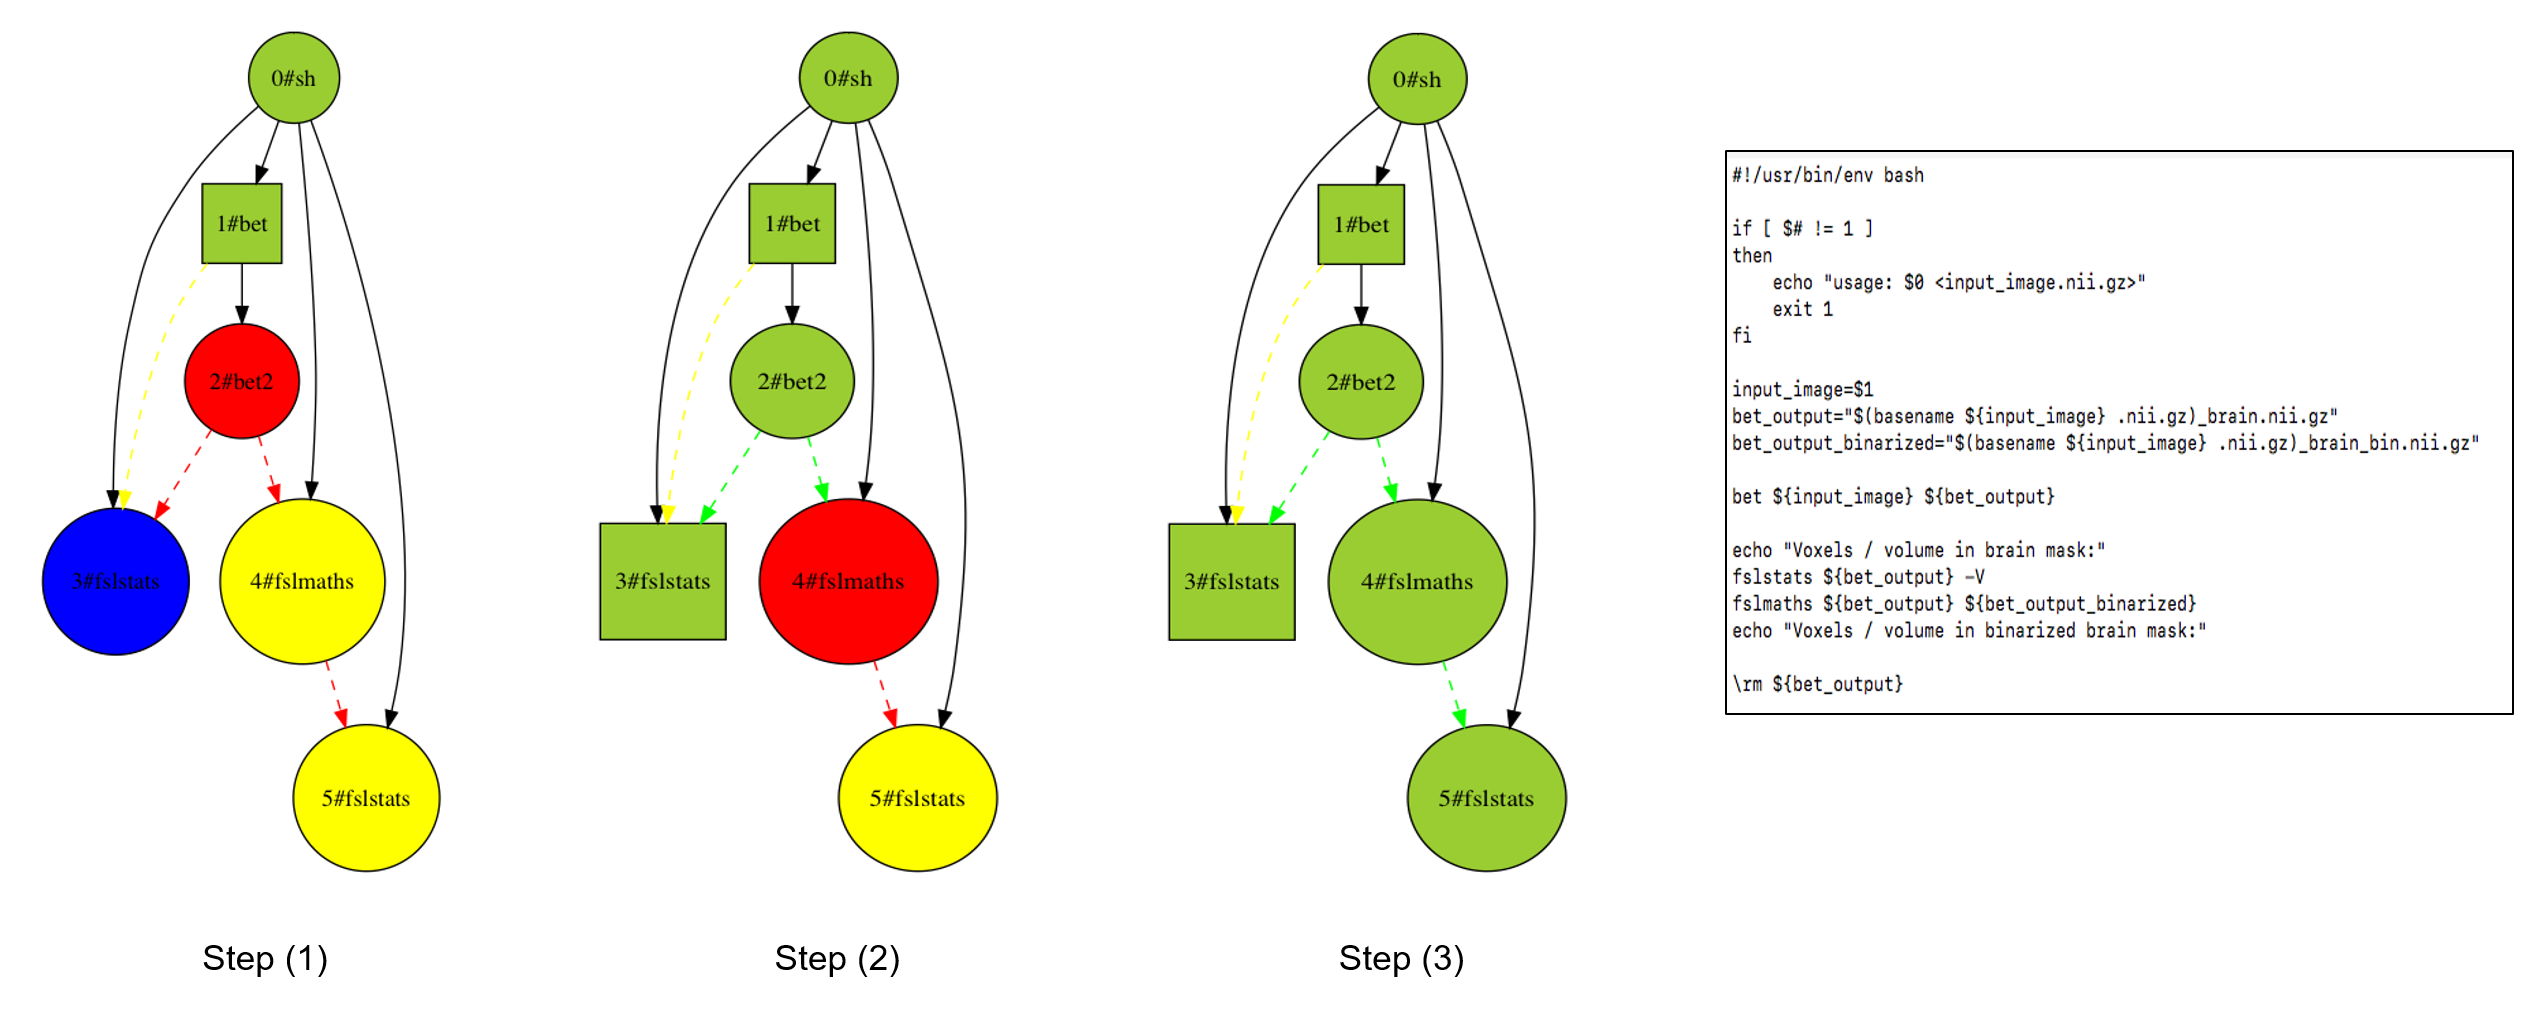
\includegraphics[width=\columnwidth]{images/iterative_modif}
  \caption{A simple example of steps of the proposed approach.}
  \label{fig:iterations}
\end{figure}

Figure~\ref{fig:iterations} illustrates our incremental labelling 
process for the example in Figure~\ref{fig:simple_script}. At every 
step, processes that created differences are shown in red and other processes 
(transparent processes) are in green. As in 
Figure~\ref{fig:simple_script}, plain black edges represent the process 
tree and dashed edges represent file dependencies: green edges 
represent files with no differences, while red edges represent files with 
differences. Temporary files are not represented because they have been 
saved as previously described.

The four steps in Figure~\ref{fig:iterations} correspond to the 
steps of the labelling algorithm. 
At step one, process \texttt{1\#bet} is executed and then labeled 
as transparent (green) as it produced files without differences.
At step 2, \texttt{2\#bet2} 
is labeled as difference creator (red) as it produced files with differences 
from files without differences. Therefore, the files produced by \texttt{2\#bet2} in  
Condition 2 are replaced with the files produced by \texttt{2\#bet2} in 
Condition 1.
At step 3, after running process \texttt{3\#fslstats}, it labeled as 
transparent as it write files without differences.
At step 4, process \texttt{4\#fslmaths} is labeled as difference creator 
as the last process of the pipeline.
As a result of these 4 steps, the final process labelling is: 
\texttt{2\#bet2} and \texttt{4\#fslmath} are difference creators (red) 
and the other processes are transparent.


\subsection{Subject clustering}

Different subjects may lead to different process tree, due to
variations that may be coming from differences in data types or
cardinality. For instance, some images may have been acquired multiple
times in some subjects. Some of these differences can be neglected, for
instance when a data decompression step is present at the beginning of the
execution for some subjects only, and other ones cannot, when different
processing paths are used in different subjects.

Different process tree shows that pipeline execution followed by a different procedure. 
This implies the possible impact of different subjects on pipeline results.
We cluster subjects into different types to specify how many different 
process trees are generated. Clustering is performed based on the process trees 
which nodes are labeled by the process name. 
In this order, 
the tree edit distance~\cite{zhang1989simple} is used as a similarity measure for 
representing the distance between labeled trees. Tree edit distance  is defined  
as the minimum number of edit operations which is needed to transform one tree into 
the other. Three edit operations are considered: node label modification, 
node removal, and node insertion. Each operation has an associated cost of 1.
With this distance, we cluster subjects using agglomerative hierarchical
clustering as implemented in SciPy~\cite{oliphant2007scipy}
(Algorithm~\ref{algo:hclustering}). As a result, the distance between
any two subjects in a cluster is lower than a threshold parameter.

Furthermore, we will show that even subjects in the same cluster, 
having the same topological process tree structure, 
may have different labels as processes that create differences.

\begin{algorithm}[h!]
\caption{Hierarchical clustering algorithm from SciPy}
\label{algo:hclustering}
\begin{algorithmic}

  \State /* Input: - a list of n trees; \texttt{T = [t${_1}$, t${_2}$,...,t${_n}$]}
  \State /*\quad \quad \quad \quad - a distance threshold value; \texttt{threshold}
  \State /* Output: a list of clusters; \texttt{C = [c${_1}$,c${_2}$,...,c${_k}$]}
  \State \texttt{\# Create a cluster for each tree in input list;}
  \State \texttt{C = [ [t${_1}$], [t${_2}$], \ldots , [t${_n}$] ]}
  \State \texttt{\# Define a 2 $\times$ 2 array to store distances}
  \State \texttt{D} = \texttt{array(n, n)}
  \While{\texttt{len(C)} > \texttt{1}}  
  \State \texttt{\# Select the two nearest clusters}
  \For{\texttt{i=1} to \texttt{n}}
  \For{\texttt{j=i+1} to \texttt{len(C)}}
  \State \texttt{D[i][j]} = $\min \left\{ \texttt{edit\_dist(a, b)}: \ \texttt{a} \in \texttt{C[i]}, \texttt{b} \in \texttt{C[j]} \right\}$
    \EndFor
  \EndFor
  \State \texttt{i, j} = $\argmin \left\{ \texttt{D[i][j]}, \ \texttt{i, j} \in \llbracket 1, \texttt{len(C)}\rrbracket^2 \right\}$
  \If{\texttt{D[i][j]} > \texttt{threshold}}
  \State \Return \texttt{C}
  \Else
  \State \texttt{\# Merge C[j] into C[i]}
  \State \texttt{C[i]} = \texttt{merge}(\texttt{C[i] and C[j]})
  \State \texttt{\# Remove C[j] from C}
  \State \texttt{remove(C[j], C)}
  \EndIf
  \EndWhile
%  \State Function edit\_distance (C${_1}$, C${_2}$)
%  \State EndFunction
\end{algorithmic}
\end{algorithm}

\section{Experiments}

In this experiment, we analyse the numerical reproducibility of the computational pipelines 
and identify the origin of differences across the operating systems. 
Two types of differences can occur in the subjects due to the differences
in the operating systems. One is between-OS differences caused by the
operating system library updates and the other type, within-OS differences
occur as a result of the pseudo-random processes used in the pipelines.

In particular, NURM-tool is tested on the neuroimaging applications which are 
predominantly using mathematical libraries. Therefore, we expect to find 
differences as a result of changing the mathematical functions between operating system libraries.

This section describes datasets and pipelines used for the analyses, 
how data processed through the pipelines, and the results.


\subsection{HCP pipelines and dataset}

We used our tool to evaluate the reproducibility of the pipelines from the Human Connectome 
Project (\href{https://www.humanconnectome.org}{HCP}).
The HCP initiative is a significant effort to acquire and analyze 
brain connectivity data from 1200 healthy adults.
It enables the neuroscience 
research community to discover relationships between brain circuits and 
individual behaviors. This helps to understand a wide range of brain disorders.
The HCP project provides (1) database services (ConnectomeDB) for storing and 
sharing primary and processed data freely, and (2) data analysis pipelines that 
are available under an open-source license.

The HCP developed a set of pre-processing pipelines to process structural,
functional, and diffusion MRI data acquired in the project. We focus on HCP
pre-processing pipelines for structural data, particularly PreFreeSurfer
and FreeSurfer. 

According to~\cite{glasser2013}, the sequence of the 
sub-pipelines in PreFreeSurfer includes 
(1) Distortion Correction (DC), 
(2) Anatomical Average (AAve), 
(3) ACPC (Anterior Commissure, Posterior Commissure) Alignment (ACPC-A), 
(4) Brain Extraction (BExt), 
(5) Bias Field Correction (BFC), 
(6) Atlas-Registration (AR).

Also, the sequence of the main sub-pipelines in FreeSurfer includes 
(1) Downsampling images, 
(2) T1w image registration, 
(3) Placement of surface images, 
(4) Folding-based surface registration.
A detailed description of the analyses done in these
pipelines is available in~\cite{glasser2013}. 

Furthermore, the average time per subject taken for PreFreeSurfer processing is 2.2 hours, 
and FreeSurfer processing is 8.3 hours (20 runs), 
and the average output file size of PreFreeSurfer processing is 2.7 GB, 
and FreeSurfer processing is 4.1 GB (20 subjects).

HCP data collected from different types of imaging techniques, including 
structural imaging (sMRI), functional imaging (fMRI), and diffusion imaging (dMRI).
The structural images include T1-weighted (T1w) and T2-weighted (T2w) images which 
help in the diagnosis of the brain injury.
The functional images, including task-based fMRI and resting-state scans, 
enable the measurement of functional activations within brain areas. 
Diffusion imaging is another kind of MRI technique, which measures 
the anatomical connectivity between regions.
See~\cite{van2013wu} for a discussion of these various terms.

Data from 1200 subjects 
is available in \href{https://db.humanconnectome.org}{the ConnectomDB repository}. 
In this paper, we randomly selected 20 unprocessed subjects from 
the HCP data release S500. All the subjects were scanned using the 3-tesla 
type of MRI scanners.


\subsection{Data processing}

We executed the pipelines using Docker containers to simplify the 
deployment of different operating system versions on execution 
platforms. 
The Docker images were built for the HCP pre-processing 
pipelines v3.19.0 (PreFreeSurfer and FreeSurfer) in 
CentOS 6.9 (Final) and CentOS 7.4 (Core). 
CentOS is a widely used operating system among the Neuroscience community because of 
the appropriate community support, network functions, safety, portability, and openness
~\cite{hanke2011neuroscience}.
These containers were installed with all the necessary software and libraries 
required to run the HCP pipelines including FSL (version 5.0.6), 
FreeSurfer (version 5.3.0-HCP, CentOS4 build), and Connectome Workbench (version 1.0).
Docker images are available on 
\href{https://hub.docker.com/r/bigdatalabteam/hcp-prefreesurfer/}{DockerHub}
for reuse.

The data were processed with PreFreeSurfer and FreeSurfer. 
First, PreFreeSurfer was utilized to analyse the unprocessed data, and then its 
results were used as the input of FreeSurfer.

Each subject was processed twice on the same operating system to detect
variability coming from pseudo-random operations. 
Within-OS variability may also be coming from other factors than pseudo-randomness. 
For instance, metadata may differ due to the presence of timestamps, 
file paths, and other execution-specific information. 
To ensure that differences belong to the file data part, 
we added distance functions specific to the file types.
These functions are \emph{mri\_diff}, \emph{mris\_diff}, and \emph{lta\_diff} 
for comparing volumes, surface-based files, 
and lta files (transforms) respectively. 
These functions compare files based on the image dimensions, 
pixel intensities, the number of vertices, and geometry information
(see~\cite{fischl2012freesurfer} for more details). 

Furthermore, we clustered subjects into different type using 
the clustering method as described before.
We set the threshold value to zero for the clustering method. 
This turns to cluster the subjects with the same topology into the same type.
Also, we used the nearest neighbor algorithm to calculate the distance between clusters.

\subsection{Results}

\subsubsection{Within-OS differences}

We didn't observe any within-OS difference in PreFreeSurfer, however, we
identified two FreeSurfer processes leading to within-OS differences due
to the use of pseudo-random numbers: image registration with
\emph{mri\_segreg}, and cortical surface curvature
estimations with \emph{mris\_curvature}. To address this issue, we fixed
the seed used by the pseudo-random number generator, through an option of
the FreeSurfer tools. In this way, our analysis can focus on between-OS
differences. 

\subsubsection{Between-OS differences in PreFreeSurfer}
%\subsubsection{PreFreeSurfer pipeline analysis} 

We identified four types of subjects with different PreFreeSurfer process
trees (Table~\ref{table:data-clusters}). Differences between subject types
are coming from different  numbers of T1 and T2 images in the raw data:
subjects of type 1 have 2 T1 images and 2 T2 images, while subjects of type
2 only have 1 T1 image and 1 T2 image. This leads to
different sets of output files. We verified that the process trees were
identical for all subjects of the same type in different versions of
CentOS.

\begin{table}
\centering
\begin{threeparttable}
\caption{Clustering of 20 input subjects.}
\label{table:data-clusters}

\begin{tabular}{@{}llllll@{}}
\toprule
Type   & Number of Subjects  & Missing File(s)                                    \\ \midrule
type1  & 9                   & None                                               \\
type2  & 7                   & [``T1w", ``T2w"]                                   \\
type3  & 2                   & [``T1w"]                                           \\
type4  & 2                   & [``T2w"]                                           \\ \bottomrule
\end{tabular}
\begin{tablenotes}
     \small
     \item *Type refers to the topology type of the process tree of subjects.
\end{tablenotes}
\end{threeparttable}
\end{table}

Figure~\ref{fig:pfs_freq} shows the frequency of the processes that create differences 
in the pipeline (the number in the bracket).
Furthermore, this figure represents the percentage of the processes that introduce 
differences along with the sub-pipelines, including linear registration 
with “\emph{FLIRT}” (in ACPC-Alignment, Brain Extraction, Distortion Correction, 
Atlas Registration), non-linear registration with “\emph{FNIRT}” (in Brain Extraction 
and Altas Registration), image warping with “\emph{new\_invwarp}” (in Brain Extraction 
and Atlas Registration). 
Besides, differences were observed in image mean and standard-deviation 
computations in image interpolation with “\emph{fslmaths}” (in Anatomical Average). 

Results show that \emph{FLIRT} is the most frequent process that produces 
differences in ACPC-Alignment across all the subjects, Distortion Correction 
in 95\% of the subjects, and Atlas Registration in 85\% of the subjects. 
In addition, there is a \emph{fslmaths} process in Anatomical Average that 
creates differences in all 11 subjects in which it has appeared.


\begin{figure}
\centering
  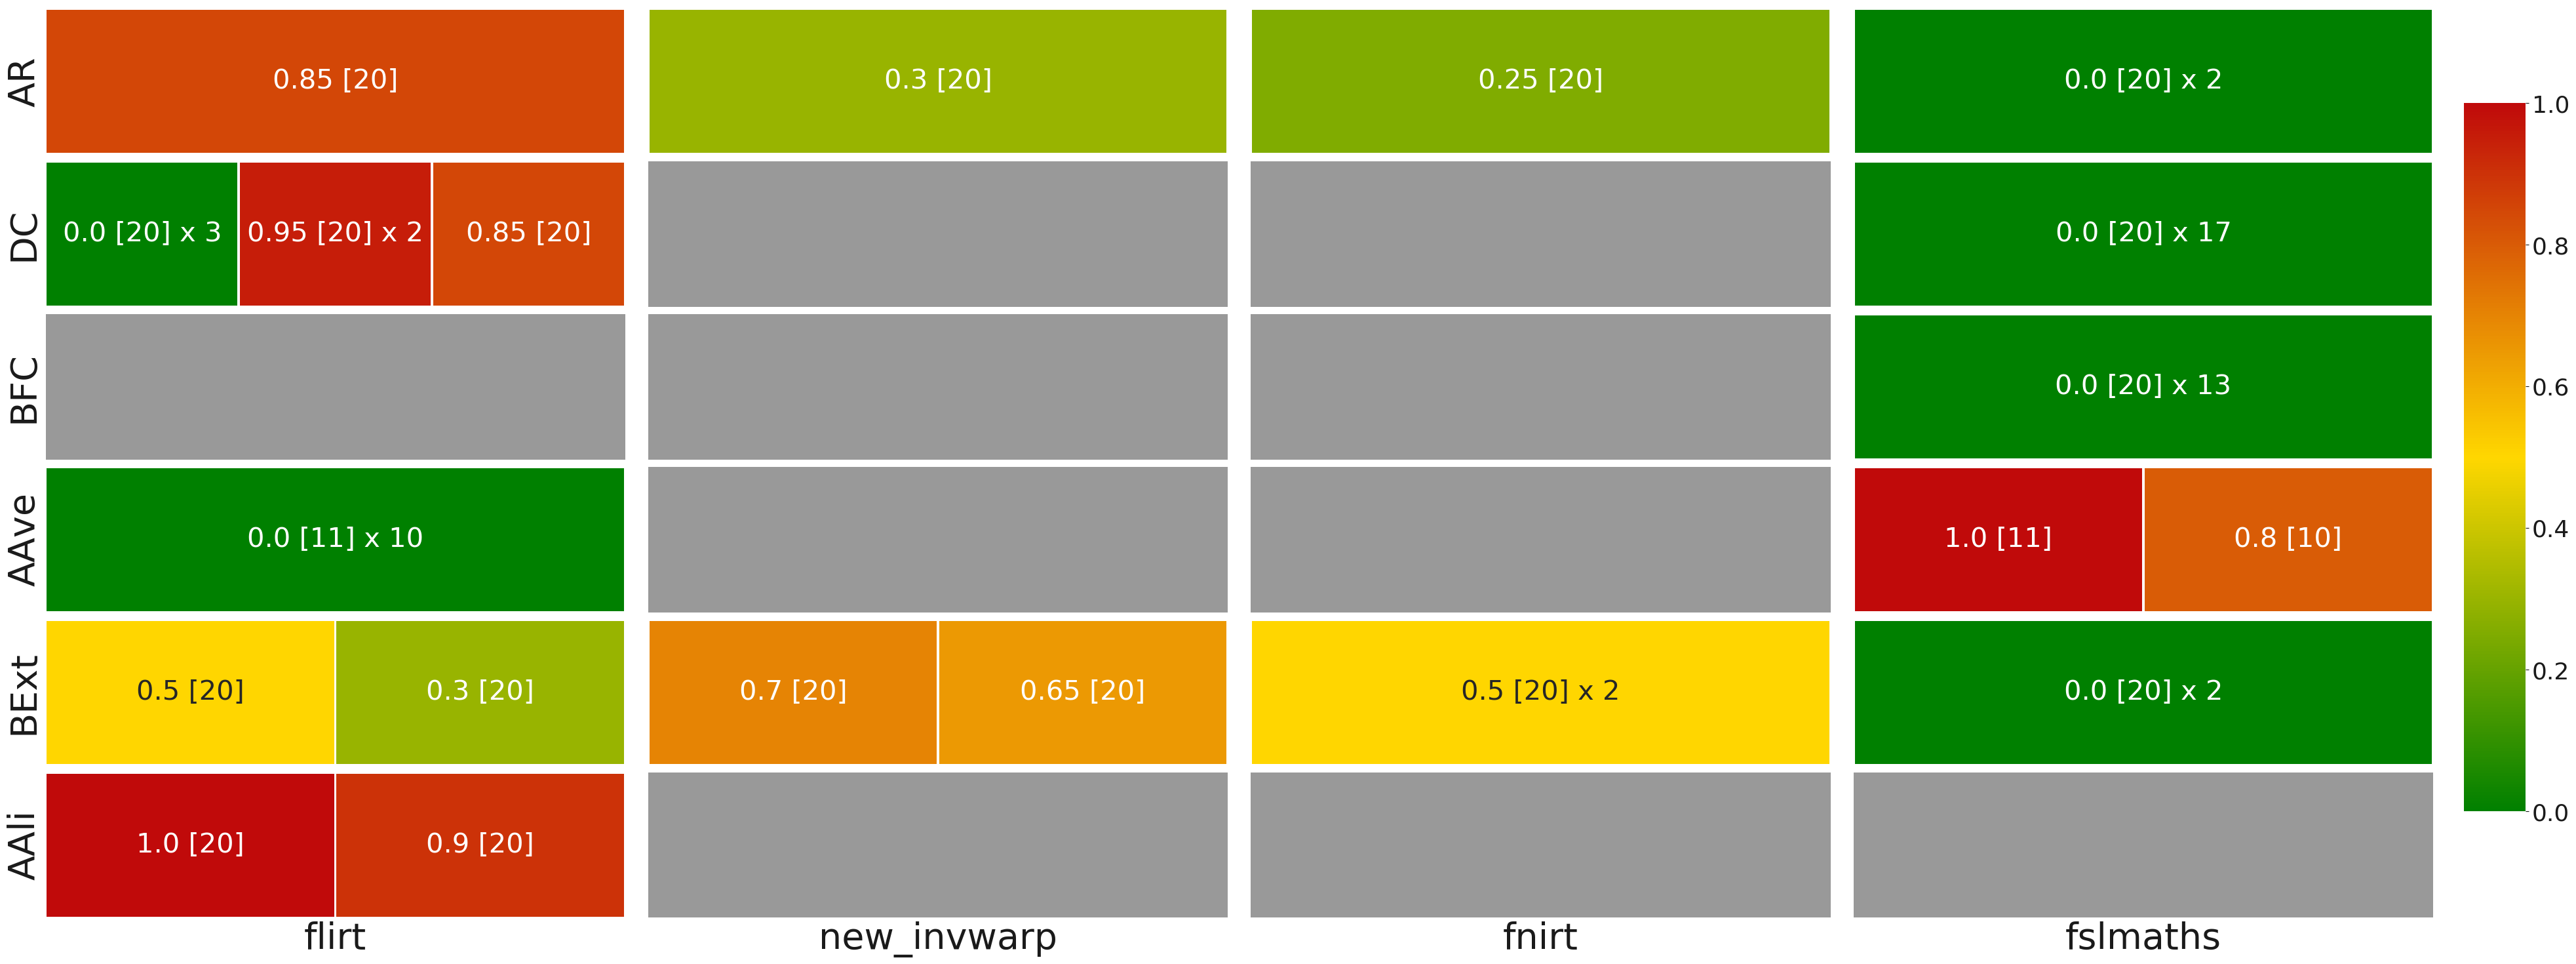
\includegraphics[width=\columnwidth]{images/pfs_heatmap.png}
  \caption{Heatmap of difference frequency of processes along with the sub-pipelines that introduce 
           differences among 20 subjects. The range between red and green colors show the most and 
           least frequency of processes respectively. Besides, the total number 
           of occurrences of each processes is represented in the bracket in each cell.}
  \label{fig:pfs_freq}
\end{figure}

To visually represent the magnitude of variations, we created checkerboard 
images from the image results of one subject in two OSes. Figure~\ref{fig:fnirt_result} 
shows the checkerboard images from the results of ACPC-Alignment in PreFreeSurfer. 
Each rectangle includes the replaced pixels with different intensity values between images.

%Alternating rectangular regions between two images, creating a characteristic 
%checkerboard-like pattern of varying magnitudes.

\begin{figure}
  \centering
    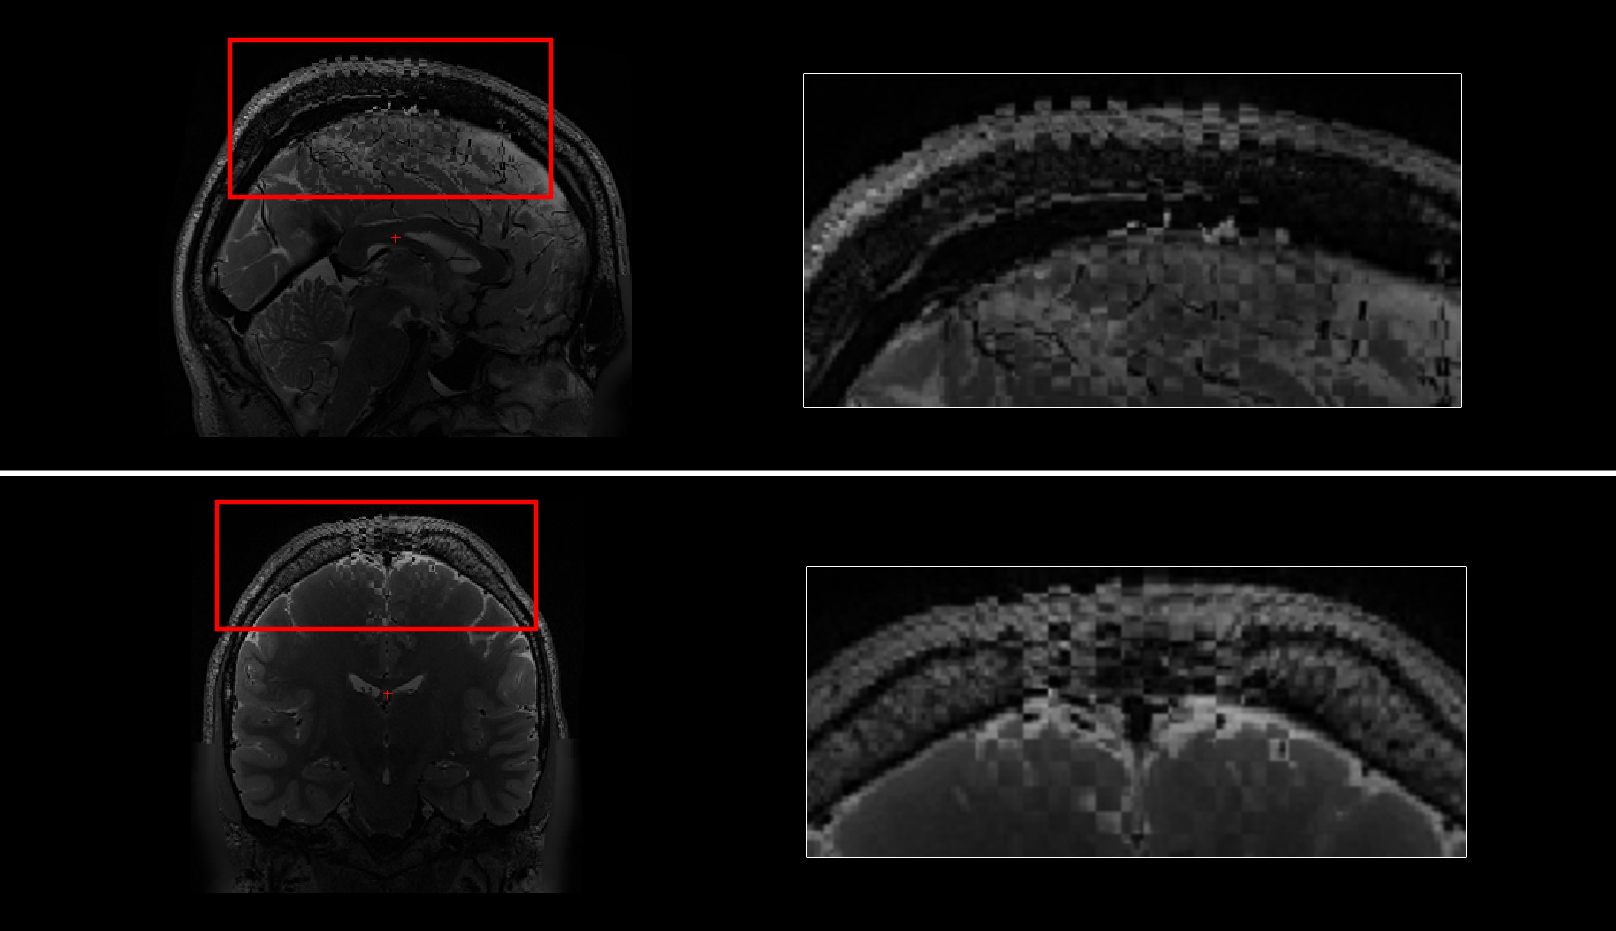
\includegraphics[width=\columnwidth]{images/segmentation.png} 
    \caption{Differences between FNIRT results of one subject from PreFreeSurfer 
    (checkerboard image \emph{T2w\_acpc\_to\_MNI\_nonli.nii.gz}) (CentOS6 vs. 
    CentOS7). Right images show the zoomed version part of the images marked 
    by the red rectangle.
    Here is 
    \href{https://raw.githubusercontent.com/ali4006/HCP-reproducibility-paper/master/images/brain_classification.gif}{the link}
    to the gif animation of the same images.
} 
    \label{fig:fnirt_result}
\end{figure}


\subsubsection{Between-OS differences in FreeSurfer} 

In the first test, the results of PreFreeSurfer on CentOS 6
feed to the FreeSurfer pipeline on both OSes. 
We fixed input data to determine whether the pipeline creates differences.
We processed 20 subjects using FreeSurfer.
NURM-tool identified \emph{mris\_make\_surfaces} as the only process in 
the pipeline that creates differences among 10 subjects.
This process generates surface files for cortical and white matter surfaces 
(see~\cite{fischl2012freesurfer} for more detail of the process). 
Also, FreeSurfer did not introduce any differences in 10 subjects. 

Results show that the static builds of FreeSurfer in which uses the embedded libraries, 
significantly avoids the creation of differences.
However, we found that between-OS differences occur when pre-processed data are different in FreeSurfer. 
For this purpose, in the second test, the results of PreFreeSurfer feed to the FreeSurfer 
pipeline on each operating system separately.
Figure~\ref{fig:tissue_class} shows between-OS differences  
as a result of propagation and amplification of differences in FreeSurfer. % that coming from PreFreeSurfer outputs. 
This figure illustrates the sum of binarized differences 
from 20 subject results of the brain tissue segmentation across OSes.
The magnitude of differences is in the range of 1-20 as the total number of subjects.

\begin{figure}
%  \includegraphics{brain\_classification}
\centering
  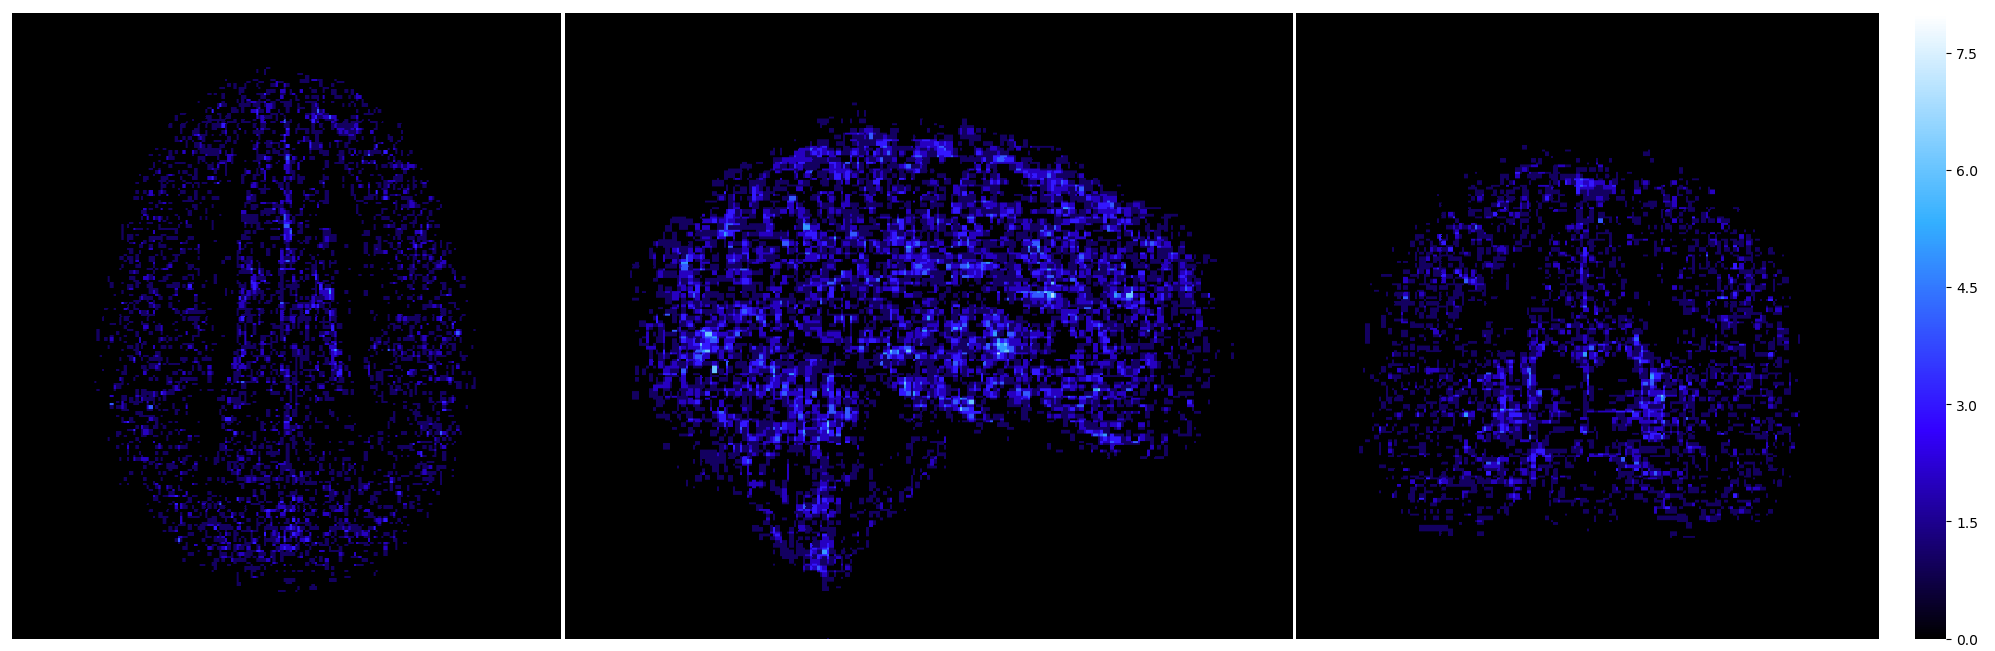
\includegraphics[width=\columnwidth]{images/brain_classification.png} 
  \caption{Heatmap binarized differences between brain segmentation results (file \emph{aseg.hires.mgz}) from 
          20 subjects in FreeSurfer (CentOS6 vs. CentOS7).} 
  \label{fig:tissue_class}
\end{figure}


\section{Discussion}

We identified four processes that create differences 
among all 28 distinct processes that are involved in the PreFreeSurfer execution. 
The numerical instability in the 
PreFreeSurfer HCP pipeline arises mainly from linear 
registration processes implemented in FSL \emph{FLIRT}. 
We can see that \emph{FLIRT} creates differences in almost all the sub-pipelines. 
Therefore, it is important to investigate the registration procedure and find 
a way to stabilize this process. 

In the second experiment, 
the analysis results obtained by the pipeline show that between-OS differences are visually substantial.
We see that statically builds of the pipeline improves reproducibility, but 
it would not improve the numerical stability of the pipeline. 
FreeSurfer pipeline propagates and amplifies the numerical differences that are created by the 
differences in the underlying operating system libraries.

In addition to variations of the operating system, other factors exist which may influence 
the reproducibility of the analyses such as software versions, compilers, hardware, etc.
Generally, we can use the Monte Carlo Arithmetic (MCA) to determine the numerical stability of the pipelines.
This algorithm perturbs every floating-point operation 
in the analysis based on the random rounding in each run. 
By this algorithm, NURM-tool can easily locate which parts of the analyzed source code are responsible 
for the floating-point related instabilities.

Although we identify the processes in the pipeline that create differences, 
the amplification of these differences should be quantified in the future works.
For this purpose, we can evaluate the final result after perturbing the identified 
processes in the pipeline iteratively.
As a result, the processes that amplify differences would have a significant effect on the results.


\section{Conclusion}

Our technique can characterize the stability of the pipelines
automatically. We identified the main causes of the between-OS differences as (1) the evolution 
of the math libraries over time and, (2) the instability of the pipelines. 
There are two ways to tackle this problem. The easy but less preferred solution is masking the instabilities.
This can be done by using, (1) single operating system for the processing of subjects, 
(2) containerizing the pipelines so that the 
processing is done on a more controlled environment, 
(3) increasing the numerical precision of the arithmetics, 
(4) building static executables by removing the host operating system library dependencies. 
These solutions only make the problem invisible, but the pipelines are stiil unstable.

The preferred solution is to find the origin of amplification of the differences and 
then fixing the particular functions/modules in the processing pipelines. 


\section{Acknowledgments}


\note{
CBRAIN team. Compute Canada(Calcul Quebec).

Data were provided by the Human Connectome Project, WU-Minn 
Consortium (Principal Investigators: David Van Essen and Kamil Ugurbil; 
1U54MH091657) funded by the 16 NIH Institutes and Centers that support 
the NIH Blueprint for Neuroscience Research; and by the McDonnell 
Center for Systems Neuroscience at Washington University.

}

% \begin{figure*}
% \centering
%   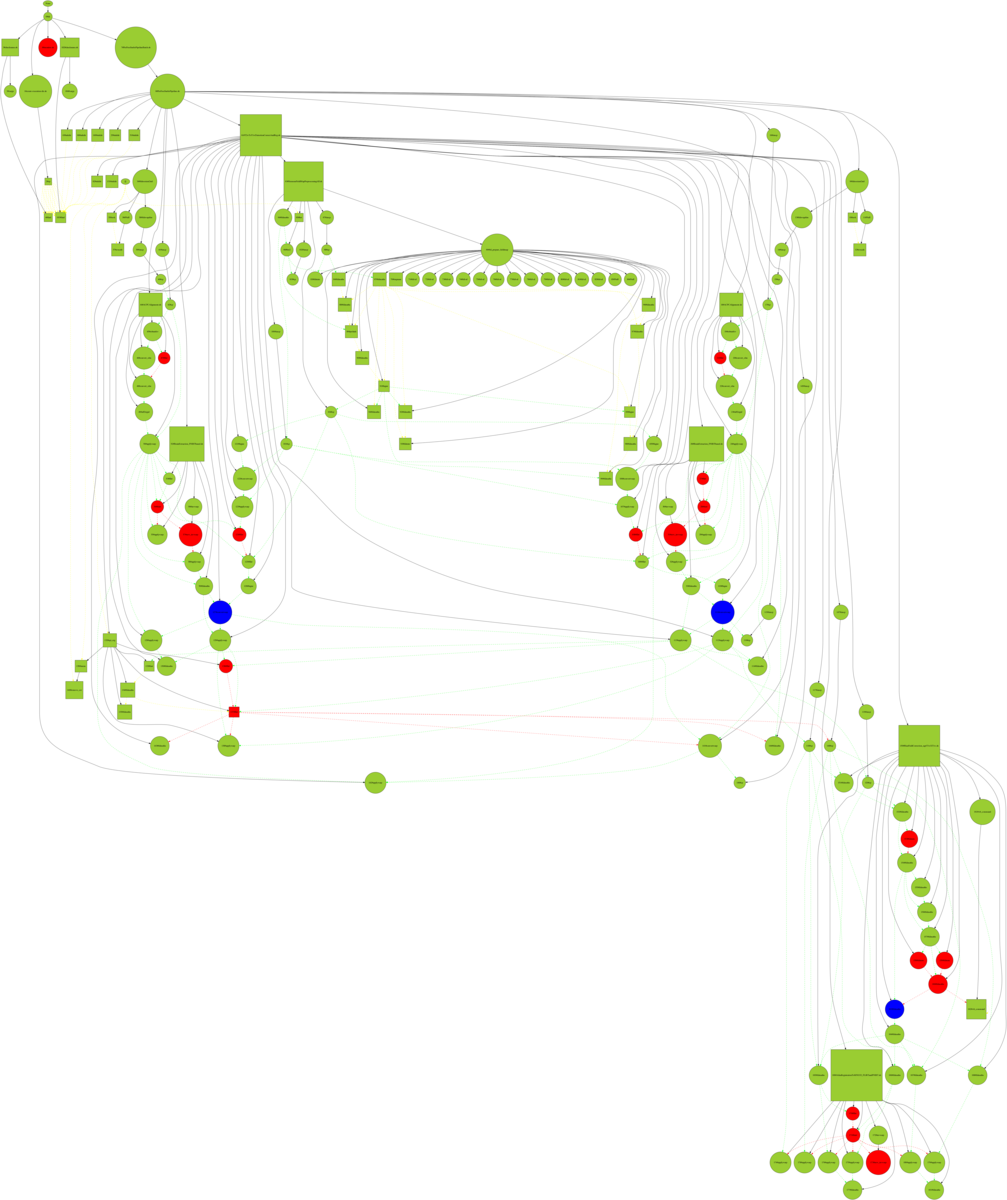
\includegraphics[width=.9\textwidth]{images/graph}
%   \caption{A complete process graph from the PreFreeSurfer pipeline.
% Full-resolution image available at \url{https://drive.google.com/open?id=174yyn8SuVOUcK5aRVw0bagjDanLD0FLt}.}
%   \label{fig:complete-graph}
% \end{figure*}

% \begin{figure*}
% \centering
%   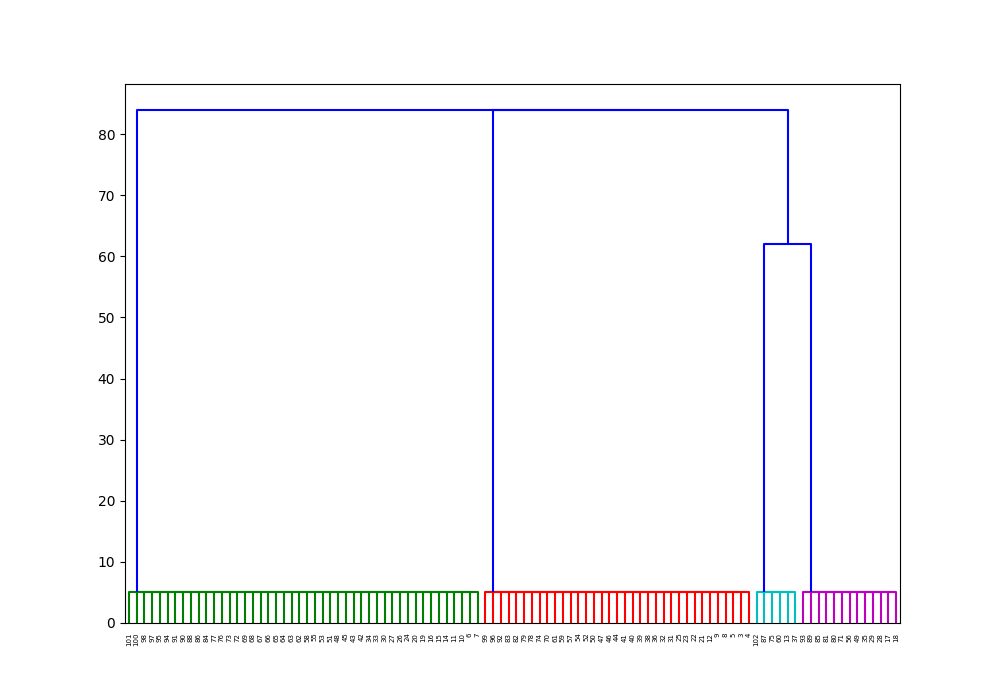
\includegraphics[width=.8\textwidth]{images/hclusters}
%   \caption{Different data types clustered among 100 subjects.}
%   \label{fig:subj-clusters}
% \end{figure*}



\bibliographystyle{plain}
\bibliography{biblio}


\end{document}
